\section{系统设计}

\subsection{系统架构设计}

TIMKE协议实现采用分层架构和模块化设计,将各功能组件高度解耦,提高系统的可维护性、可测试性和可扩展性。整体架构分为五个核心层次,如图\ref{fig:system-architecture}所示:

\begin{figure}[H]
  \centering
  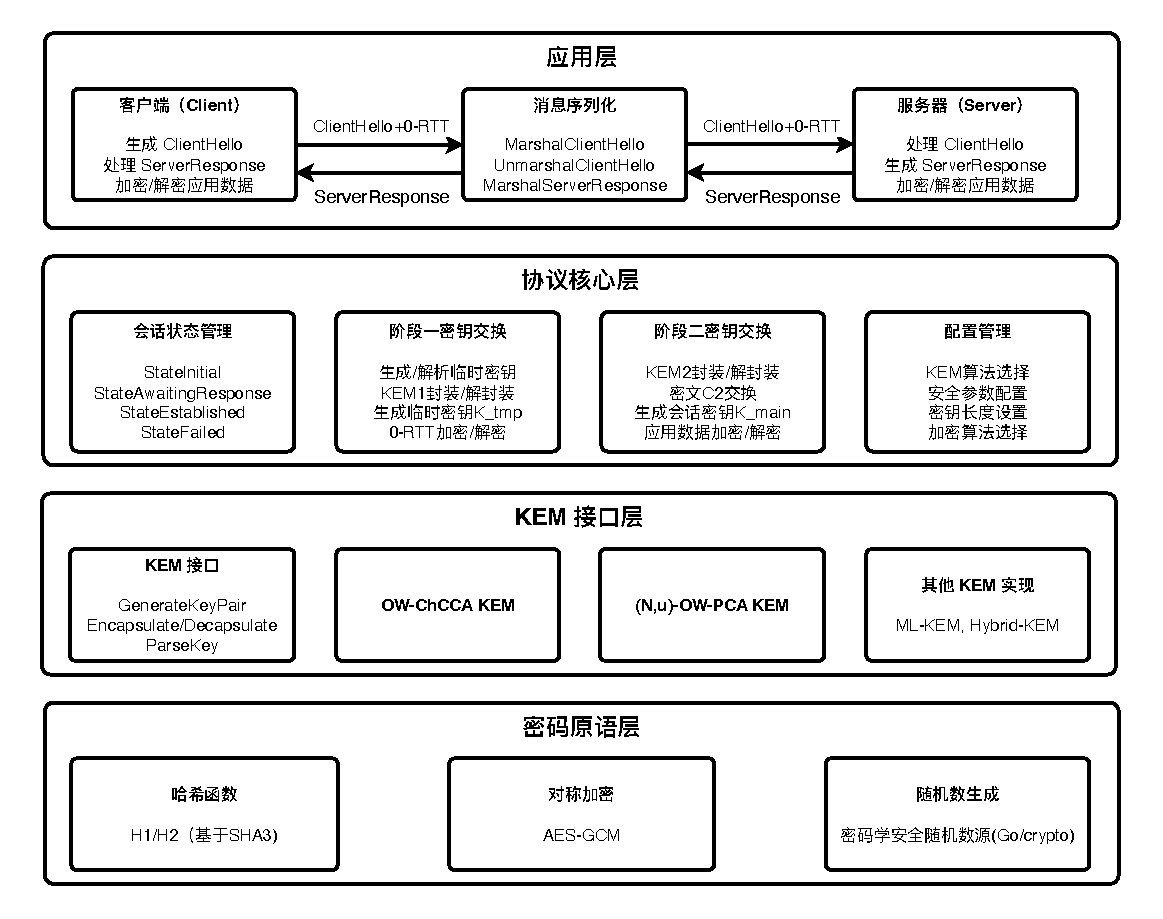
\includegraphics[width=0.9\textwidth]{figures/implementation.drawio.pdf}
  \caption{TIMKE协议实现架构}
  \label{fig:system-architecture}
\end{figure}

\subsubsection{应用层}
应用层提供用户界面和演示功能,封装了Client和Server实体,支持完整的协议交互和0-RTT数据传输。该层主要由以下组件构成:

\begin{itemize}
    \item \textbf{客户端程序}:负责启动密钥交换流程、发送0-RTT数据并与服务器进行加密通信,支持交互式和批处理两种运行模式。
    
    \item \textbf{服务器程序}:负责接收连接请求、处理密钥协商消息并响应客户端,支持多客户端并发连接。
    
    \item \textbf{演示脚本}:提供用户友好的命令行界面,自动化协议测试流程,让用户无需了解底层实现细节即可体验协议功能。
\end{itemize}

\subsubsection{序列化层}
序列化层负责协议消息的编码与解码,确保跨平台通信的一致性和正确性。主要组件包括:

\begin{itemize}
    \item \textbf{消息定义}:定义ClientHello和ServerResponse两种主要消息结构,包含必要的协议字段和可选扩展。
    
    \item \textbf{编码/解码器}:实现二进制格式的消息序列化和反序列化,使用长度前缀和稠密编码优化通信效率。
    
    \item \textbf{协议协商支持}:通过消息字段支持KEM类型协商,允许客户端和服务器动态选择兼容的加密算法。
\end{itemize}

\subsubsection{协议核心层}
协议核心层实现TIMKE协议的状态管理、会话处理和密钥协商逻辑,是整个系统的核心。主要组件包括:

\begin{itemize}
    \item \textbf{会话状态管理}:定义并管理协议的四种核心状态(Initial、AwaitingServerResponse、Established、Failed),确保协议操作顺序和安全性。
    
    \item \textbf{阶段一密钥交换}:实现临时会话密钥的协商和0-RTT数据的加密/解密,支持初始连接的低延迟通信。
    
    \item \textbf{阶段二密钥交换}:实现具有弱前向安全性的主会话密钥协商,用于后续通信的高强度安全保障。
    
    \item \textbf{配置管理}:处理KEM算法选择、安全参数配置等协议设置,支持灵活的部署选项。
\end{itemize}

\subsubsection{KEM接口层}
KEM接口层定义统一的密钥封装机制接口,实现算法无关的操作抽象,允许协议灵活嵌入不同的KEM实现。主要组件包括:

\begin{itemize}
    \item \textbf{KEM接口定义}:规范化的KEM操作集,包括密钥生成、封装、解封装等核心功能。
    
    \item \textbf{OW-ChCCA KEM实现}:基于格密码学的单向可检测选择密文安全KEM实现,是协议安全证明的直接对应。
    
    \item \textbf{ML-KEM集成}:集成NIST标准的后量子KEM算法,提供高效的实用替代方案。
    
    \item \textbf{KEM注册表}:通过工厂模式和注册表模式管理不同KEM算法,支持运行时动态选择。
\end{itemize}

\subsubsection{密码原语层}
密码原语层提供哈希函数、对称加密等基础密码学功能,为协议的密钥派生和数据加密提供支持。主要组件包括:

\begin{itemize}
    \item \textbf{哈希函数}:基于SHA3实现的H1和H2密钥派生函数,支持临时会话密钥和主会话密钥的安全派生。
    
    \item \textbf{对称加密}:基于AES-GCM的加密方案,为0-RTT数据和后续通信提供机密性和完整性保护。
    
    \item \textbf{随机数生成}:密码学安全的随机数源,用于密钥生成和防重放保护。
\end{itemize}

这种分层设计严格遵循关注点分离原则,使各组件能够独立演化和测试。同时,通过定义清晰的接口,系统支持在不修改协议核心逻辑的情况下替换或更新各层组件,为协议的长期维护和演进奠定了坚实基础。

\subsection{功能模块设计}

\subsubsection{协议参与方与工作流程}

TIMKE协议涉及两个参与方:客户端(C)和服务器(S),它们通过两个阶段的交互完成密钥协商。整体工作流程如图\ref{fig:protocol-flow}所示:

\begin{figure}[H]
  \centering
  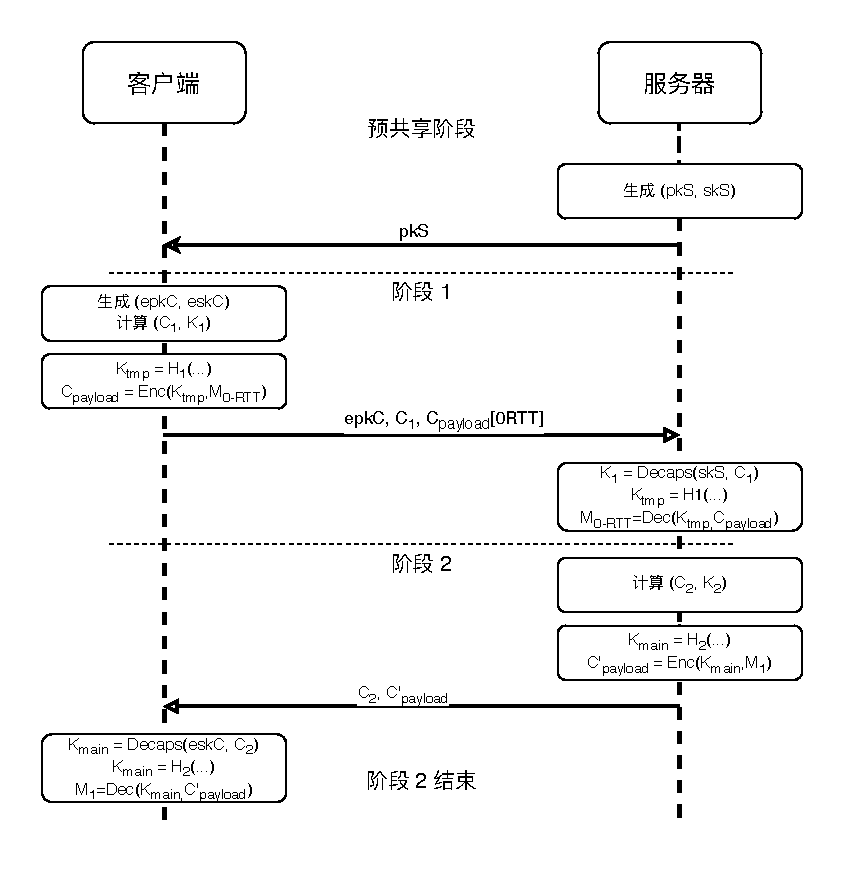
\includegraphics[width=0.8\textwidth]{figures/protocol.drawio.pdf}
  \caption{TIMKE协议工作流程}
  \label{fig:protocol-flow}
\end{figure}

\paragraph{预共享阶段}
在正式协议交互前,服务器生成长期密钥对$(pk_S, sk_S)$,并通过可信渠道将公钥$pk_S$分发给客户端。这一阶段类似于TLS中的证书分发过程。

\paragraph{第一阶段:临时密钥协商与0-RTT传输}
\begin{enumerate}
    \item 客户端生成临时密钥对$(epk_C, esk_C)$并使用服务器公钥封装共享密钥$(C_1, K_1)$
    \item 客户端派生临时会话密钥$K_{tmp} = H_1(pk_S, C_1, K_1)$
    \item 客户端使用$K_{tmp}$加密0-RTT数据$C_{payload}$并发送$(epk_C, C_1, C_{payload})$
    \item 服务器使用私钥解封装得到$K_1$,派生相同的$K_{tmp}$并解密0-RTT数据
\end{enumerate}

\paragraph{第二阶段:主会话密钥建立}
\begin{enumerate}
    \item 服务器使用客户端临时公钥封装共享密钥$(C_2, K_2)$
    \item 服务器派生主会话密钥$K_{main} = H_2(pk_S, epk_C, C_1, C_2, K_1, K_2)$
    \item 服务器加密应用数据并发送$(C_2, C'_{payload})$
    \item 客户端解封装得到$K_2$,派生相同的$K_{main}$并解密服务器数据
\end{enumerate}

\subsubsection{密钥封装机制实现}

作为TIMKE协议的核心组件,系统实现了两类KEM算法:

\paragraph{OW-ChCCA KEM}
单向可检测选择密文安全KEM是TIMKE协议安全证明的基础,基于格密码学构建,具体实现包括:

\begin{itemize}
    \item \textbf{密钥结构}:公钥包含矩阵$\mathbf{A}$、$\mathbf{u}_0$、$\mathbf{u}_1$;私钥包含矩阵$\mathbf{Z}_b$和标志位$b$
    \item \textbf{密钥生成}:从均匀分布随机采样$\mathbf{A}$,从高斯分布采样$\mathbf{Z}_b$,计算$\mathbf{A}\mathbf{Z}_b$
    \item \textbf{封装/解封装}:基于学习带误差(LWE)问题构建的安全机制
    \item \textbf{参数优化}:针对实际应用环境,调整理论参数以平衡安全性和性能
\end{itemize}

\paragraph{ML-KEM集成}
为提供更高效的实现方案,系统集成了NIST标准的ML-KEM算法:

\begin{itemize}
    \item \textbf{支持级别}:ML-KEM-512(AES-128等效安全级别)、ML-KEM-768(AES-192等效)、ML-KEM-1024(AES-256等效)
    \item \textbf{接口适配}:通过统一KEM接口封装ML-KEM操作,实现无缝集成
    \item \textbf{性能优化}:利用ML-KEM的高效实现提升整体协议性能
\end{itemize}

\subsubsection{消息格式与处理}

系统定义了两种主要消息类型,用于客户端和服务器之间的交互:

\paragraph{ClientHello消息}
客户端发送的第一个消息,包含以下字段:
\begin{itemize}
    \item \textbf{EphemeralPublicKey}:客户端临时公钥$epk_C$
    \item \textbf{Ciphertext1}:使用服务器公钥封装的密文$C_1$
    \item \textbf{EncryptedPayload}:使用临时会话密钥加密的0-RTT数据(可选)
    \item \textbf{KEM1Type/KEM2Type}:用于指示使用的KEM类型(用于协商)
\end{itemize}

\paragraph{ServerResponse消息}
服务器对ClientHello的响应,包含以下字段:
\begin{itemize}
    \item \textbf{Ciphertext2}:使用客户端临时公钥封装的密文$C_2$
    \item \textbf{EncryptedPayload}:使用主会话密钥加密的应用数据(可选)
\end{itemize}

消息序列化采用长度前缀编码方式,确保跨平台兼容性和传输效率。

\subsubsection{会话状态管理}

系统采用状态机模式管理协议状态,定义了四种核心状态:

\begin{itemize}
    \item \textbf{StateInitial}:初始状态,表示会话尚未开始
    \item \textbf{StateAwaitingServerResponse}:客户端已发送请求,等待服务器响应
    \item \textbf{StateEstablished}:会话成功建立,可以安全通信
    \item \textbf{StateFailed}:会话建立失败,需要重新协商
\end{itemize}

状态转换逻辑确保协议严格按照预定流程执行,防止状态错误导致的安全问题。每个状态转换都包含完整的错误处理逻辑,保证在异常情况下能够正确回退或终止会话。

\subsubsection{密钥派生机制}

协议中的密钥派生是安全性的关键环节,实现了两个专用的密钥派生函数:

\begin{itemize}
    \item \textbf{H1函数}:派生临时会话密钥,$K_{tmp} = H_1(pk_S, C_1, K_1)$
    \item \textbf{H2函数}:派生主会话密钥,$K_{main} = H_2(pk_S, epk_C, C_1, C_2, K_1, K_2)$
\end{itemize}

这些函数基于SHA3-512哈希函数实现,采用域分隔技术增强安全性,确保不同上下文的哈希值不会发生冲突。密钥派生过程包括完整的输入验证,确保不会处理无效数据。

\subsubsection{扩展性与配置机制}

系统设计重视扩展性与灵活配置,提供多层次的配置接口:

\begin{itemize}
    \item \textbf{KEM算法配置}:支持多种KEM组合,如ML-KEM-768/1024或OWChCCA/ML-KEM混合
    \item \textbf{安全参数选择}:允许根据应用需求选择不同安全级别
    \item \textbf{会话选项配置}:通过SessionOptions接口灵活配置会话参数
\end{itemize}

所有核心组件均通过接口定义,支持替换具体实现。系统使用注册机制管理KEM算法,便于添加新的算法实现。这种设计确保系统能够随着密码学研究进展和安全需求变化而演进,延长协议实现的生命周期。